\documentclass[11pt,a4paper]{article}
\usepackage[T1]{fontenc}
\usepackage[utf8]{inputenc}
\usepackage{mathpazo}
\usepackage[scaled=.92]{helvet}
\usepackage{microtype,amsmath,amssymb,amsthm,booktabs,array,tabularx,longtable}
\usepackage[a4paper,margin=25mm,headheight=15pt]{geometry}
\usepackage{xcolor,graphicx,tikz,pgfplots,tcolorbox,enumitem,fancyhdr,lastpage}
\usetikzlibrary{arrows.meta,positioning,calc,fit,backgrounds}
\pgfplotsset{compat=1.18}
\usepackage{titlesec}
\usepackage[section]{placeins}
\usepackage[numbers,sort&compress]{natbib}
\usepackage{hyperref}
\definecolor{ink}{HTML}{201B2B}
\definecolor{gold}{HTML}{A36B15}
\definecolor{wine}{HTML}{721D50}
\definecolor{cream}{HTML}{FAF6ED}
\definecolor{muted}{HTML}{565363}
\hypersetup{colorlinks=true,linkcolor=wine,citecolor=wine,urlcolor=wine,pdftitle={SUCCESSOR Omega: The Institution That Compounds},pdfauthor={Vincent Boucher},pdfsubject={Transformational Intelligence; mission advantage; institutional succession; productive capacity},pdfkeywords={SUCCESSOR Omega, AGI ALPHA, Transformational Intelligence, capability inheritance, renewal-adjusted Alpha}}
\urlstyle{same}
\titleformat{\section}{\Large\sffamily\bfseries\color{ink}}{\thesection}{.6em}{}
\titleformat{\subsection}{\large\sffamily\bfseries\color{ink}}{\thesubsection}{.6em}{}
\titleformat{\subsubsection}{\sffamily\bfseries\color{ink}}{\thesubsubsection}{.6em}{}
\setlength{\parindent}{0pt}
\setlength{\parskip}{6pt}
\widowpenalty=10000
\clubpenalty=10000
\displaywidowpenalty=10000
\setlength{\emergencystretch}{2em}
\setlist{nosep,leftmargin=1.4em}
\newtheorem{proposition}{Proposition}
\newtheorem{definition}{Definition}
\newtheorem{corollary}{Corollary}
\newcommand{\Om}{\ensuremath{\Omega}}
\newcommand{\R}{\mathbb{R}}
\newcommand{\E}{\mathbb{E}}
\newcommand{\spec}{\textsc{Specialist ASI}}
\newtcolorbox{insight}[1][]{colback=cream,colframe=gold,boxrule=.6pt,arc=1mm,left=3mm,right=3mm,top=2mm,bottom=2mm,title=#1,coltitle=ink,colbacktitle=cream,fonttitle=\sffamily\bfseries}
\pagestyle{fancy}
\fancyhf{}
\fancyhead[L]{\small\sffamily SUCCESSOR \Om}
\fancyhead[R]{\small\sffamily The Institution That Compounds}
\fancyfoot[L]{\footnotesize\sffamily Research edition 1.1.0 \;\textbullet\; 3 November 2026}
\fancyfoot[R]{\footnotesize\sffamily\thepage\,/\,\pageref{LastPage}}
\renewcommand{\headrulewidth}{.3pt}
\makeatletter
\newcommand{\inputrows}[1]{\@@input#1 }
\makeatother
\input{generated.tex}
\begin{document}
\hypersetup{pageanchor=false}
\begin{titlepage}
\color{ink}
\vspace*{3mm}
{\sffamily\small\color{gold} MONTREAL.AI\quad /\quad QUEBEC.AI\hfill RESEARCH EDITION 1.1.0}\par
\vspace{17mm}
{\sffamily\small\bfseries\color{wine} TRANSFORMATIONAL INTELLIGENCE $\boldsymbol{\infty}$}\par
\vspace{5mm}
{\fontsize{43}{47}\selectfont SUCCESSOR $\boldsymbol{\Omega}$}\par
\vspace{5mm}
{\fontsize{29}{35}\selectfont\bfseries The Institution\\That Compounds\par}
\vspace{8mm}
{\large Manufacturing mission advantage, preserving inventive capability, and financing the physical frontier}\par
\vspace{10mm}
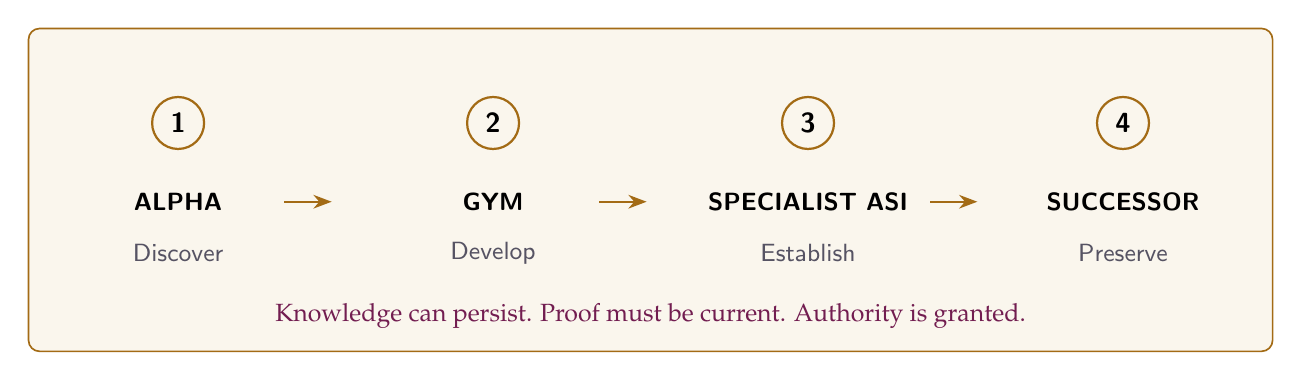
\begin{tikzpicture}[x=1cm,y=1cm]
\fill[cream,rounded corners=4pt] (0,0) rectangle (15.8,4.1);
\draw[gold,line width=.6pt,rounded corners=4pt] (0,0) rectangle (15.8,4.1);
\foreach \x/\n/\lab/\sub in {1.9/1/ALPHA/Discover,5.9/2/GYM/Develop,9.9/3/SPECIALIST ASI/Establish,13.9/4/SUCCESSOR/Preserve} {
\draw[gold,thick] (\x,2.9) circle(.33);
\node[font=\sffamily\bfseries] at (\x,2.9) {\n};
\node[font=\sffamily\bfseries\small] at (\x,1.9) {\lab};
\node[font=\sffamily\small,text=muted] at (\x,1.25) {\sub};
}
\foreach \x in {3.25,7.25,11.45}{\draw[-{Stealth},gold,thick] (\x,1.9)--(\x+.6,1.9);}
\node[font=\small,text=wine] at (7.9,.45) {Knowledge can persist. Proof must be current. Authority is granted.};
\end{tikzpicture}\par
\vspace{6mm}
{\large\itshape The enduring advantage is not a model.\\[2pt]It is the ability to make the next model useful.\par}
\vfill
{\large\bfseries Vincent Boucher}\par
{\sffamily MONTREAL.AI \;\textbullet\; QUEBEC.AI}\par
{3 November 2026}\par
\vspace{8mm}
{\small\color{muted} A constructive research framework, an exact finite renewal study, and a local authorization-state witness. Not a claim of achieved superintelligence, measured customer profit, or installed physical capacity.}\par
\vspace{5mm}
{\sffamily\bfseries\color{gold} OWN THE INSTITUTION. REPLACE THE MODELS. PRESERVE THE MISSION.}
\end{titlepage}
\hypersetup{pageanchor=true}
\begin{abstract}
A breakthrough can leave its owner with a result but without a renewable means of producing the next one. We propose a customer-owned mission institution that preserves methods, instruments, skills, and operating memory across model and supplier changes while renewing evidence and receiving authority separately. We define \emph{renewal-adjusted Alpha}: complete-horizon comparative mission advantage including construction, unsuccessful search, operation, replacement, requalification, and residual obligations. An exact authored cash-constrained example exhibits a lifecycle reversal: a lower-contribution portable capability yields 230 units of cash surplus versus 200 for repeated reconstruction. An ordinary planner with the same choices ties the result, so this is a mechanism contrast rather than demonstrated superiority over the strongest complete alternative. All 324 optimizer--oracle comparisons across 162 deterministic environments agree. A separately disclosed unknown-schedule extension adds 96 environments and 192 exact comparisons: portability helps none of 48 eight-period cases and one of 48 sixteen-period cases; that positive case also has worse downside. We correct a temporal defect in the local authorization witness and expand its accompanying regression suite. The resulting contribution is a scoped institutional framework, reproducible conditional studies, and a proposed Industrial Requalification Foundry. We connect useful inheritance and earned resources to qualified physical construction without equating financial accumulation with installed capacity. Autonomous discovery, real customer profitability, general ASI, and stellar-scale deployment remain unestablished by these studies.
\end{abstract}
\begin{insight}[The paper in one sentence]
Build advantages worth proving; preserve the machinery that makes them renewable; spend only resources actually available; and make every transition into greater productive capacity earn its own evidence.
\end{insight}
\subsection*{Reader's map}
Sections 1--3 explain the institution and its four public stages. Sections 4--6 define the evidence boundary, economic objective, and exact results. Sections 7--9 develop renewal, inventive succession, and physical expansion. Sections 10--12 give an actionable industrial research programme, limitations, and the conclusion. The appendices provide proofs, a complete numerical specification, an evidence ledger, and reproduction instructions.
\clearpage
\setcounter{tocdepth}{1}
\tableofcontents
\clearpage
\section*{The thesis at a glance}
\addcontentsline{toc}{section}{The thesis at a glance}
\begin{insight}[Do not merely own a result. Own a renewable means of making results.]
A model can be replaced. An institution should preserve the mission, the legitimate learning, and the ability to establish what works next. Its retained assets earn their place by improving fresh work after their full lifecycle burden.
\end{insight}

\textbf{What compounds.} Useful methods, executable instruments, applicability knowledge, and tested constructors can make subsequent capabilities less costly or newly reachable. Earned cash can finance that work. These are different enabling relationships, each requiring its own evidence.

\textbf{What does not transfer automatically.} Current proof, credentials, customer consent, and operating authority do not become valid merely because a predecessor possessed them. A supplier change may preserve the source while invalidating the warrant to use it.

\textbf{What the exact study establishes.} In one known-schedule fixture, the portable route produces 230 rather than 200 units of cash surplus. A competent ordinary planner with the same choices ties it. Under unannounced changes, most tested environments yield no portability benefit; the one positive 16-period case also exposes greater downside. The mechanism is conditional continuity value, not a new level of AI capability.

\textbf{What the institution should construct next.} The proposed Industrial Requalification Foundry targets a missing productive means: a reliable way to identify which consequential claims a change invalidates, construct the necessary new experiments, and preserve only evidence that remains applicable. That instrument must beat strong complete alternatives before it becomes a product claim.

\textbf{Where this could lead.} Accepted value can fund scientific instruments, manufacturing systems, and energy capacity through independently qualified construction. The physical frontier advances when machinery works and obligations are met, not when a forecast assigns it a large valuation.

\begin{center}
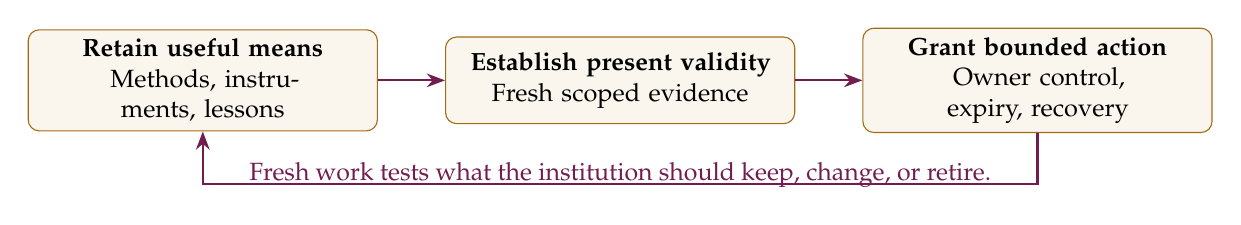
\begin{tikzpicture}[box/.style={draw=gold,fill=cream,rounded corners,align=center,text width=4.2cm,minimum height=1.1cm,font=\small},arr/.style={-{Stealth},thick,wine}]
\node[box] (k) at (0,0) {\textbf{Retain useful means}\\Methods, instruments, lessons};
\node[box] (e) at (5.3,0) {\textbf{Establish present validity}\\Fresh scoped evidence};
\node[box] (a) at (10.6,0) {\textbf{Grant bounded action}\\Owner control, expiry, recovery};
\draw[arr] (k)--(e);\draw[arr] (e)--(a);
\draw[arr] (a.south) -- ++(0,-.65) -| (k.south);
\node[font=\small,text=wine] at (5.3,-1.2) {Fresh work tests what the institution should keep, change, or retire.};
\end{tikzpicture}
\end{center}

\textbf{The contribution in context.} Lifecycle costing, finite dynamic programming, and validity intervals are established methods. The proposed synthesis joins them to mission-specific evidence, customer-controlled succession, generative inheritance, and explicit physical expansion. The contribution is that inspectable construction and research programme---not priority for the component methods or an empirical demonstration of the full ambition.

\begin{center}\large\itshape
The institution is not the archive.\\[3pt]
It is the ability to turn legitimate inheritance into useful next action.
\end{center}
\clearpage

\section{From a successful answer to an enduring institution}
\label{sec:institution}
The economically important question is not only whether an intelligence can produce an excellent result. It is whether an owner can reliably obtain further valuable results after the underlying model, operating environment, commercial relationship, or mission requirement changes. A system that wins once but cannot be renewed may be less useful than a slightly weaker system that can preserve, adapt, and re-establish what made its work valuable.

This paper develops \emph{SUCCESSOR $\Omega$} as a proposed institution of mission intelligence. The institution is not a particular model. It is the maintained arrangement through which legitimate knowledge, executable methods, evaluation, and bounded authority serve an enduring purpose. Models are replaceable contributors. They are not the institution's identity, its accumulated evidence, or its right to act.

The founding distinction comes from Transformational Intelligence: the authorized purpose, the current formulation of a problem, and the instrument used to evaluate a result are different objects \citep{boucherTI}. A method can change without changing the purpose. A new evaluator requires separate justification. A better-looking score cannot authorize the builder to redefine success. Here we apply that distinction across time: the institution should preserve what remains useful without preserving every assumption, dependency, or permission of the system that originally produced it.

\begin{insight}[The continuity principle]
Continuity is not the refusal to change. It is the ability to change components without losing the mission, legitimate knowledge, or accountability for what has been done.
\end{insight}

\subsection{What this paper adds}
The earlier FLYWHEEL $\Omega$ studies how production and verification change feasible economic interactions, including the cash timing that finances subsequent work \citep{boucherFlywheel}. SUPER ALPHA connects viable productive arrangements to value capture and successive capability construction \citep{boucherSuper}. The present paper addresses a different bottleneck: \emph{what survives replacement, and when paying to preserve it is worthwhile}.

Mission-relative revalidation in the earlier Transformational Autonomous Enterprises separates reusable generic checks from fresh mission validation; its direct specialist remains a strong comparator \citep{boucherEnterprise}. Out-Reflect constructs fault-bounded self-correcting reference evidence within a declared mathematical family \citep{boucherReflect}. We inherit those distinctions rather than treating a retained certificate or agreeing models as sufficient truth.

We make four concrete additions. First, renewal-adjusted Alpha evaluates an advantage over the lifecycle in which it must remain usable, rather than at one model release. Second, a context-bound succession contract separates portable knowledge from current evidence and authority. Third, an exact finite study identifies when a portability investment beats repeated rebuilding, when it does not, and why a competent ordinary planner can reproduce the result. Fourth, a physical-expansion contract makes the conversion of cash and knowledge into commissioned capacity inspectable rather than automatic.

These are a framework, conditional mathematical results, and newly executed software evidence. The full institutional architecture and industrial programme remain proposed. The public conceptual vocabulary has been synthesized from the author's programme materials; the private working conversations and supplied visual source files are not redistributed. Earlier public papers provide the stable citable foundation. This is a research edition, not a claim of independent peer review.

\subsection{The opportunity is more than continuity software}
The consequential target is the construction of productive capabilities that organizations cannot currently sustain economically. A laboratory might discover a useful process but repeatedly lose the ability to qualify it after instruments change. An industrial operator might possess excellent models but no portable, testable representation of operating conditions. A group of specialists might solve individual tasks yet fail at the interfaces required for a complete customer outcome.

The institution should therefore search over representations, experimental instruments, interfaces, production sequences, commercial commitments, and coordination arrangements. It may discover that the best move is a conventional method, a smaller system, or no investment. An institution exists to make valuable work possible, not to make itself indispensable.

The long-horizon ambition is correspondingly larger than retaining a chat history. It is to turn successful intelligence into accumulated scientific and productive means, and to use genuinely earned resources to build what the next consequential objective requires. Every step must preserve the difference between a plausible opportunity and a commissioned capability.

\section{The architecture of ownership}
\label{sec:ownership}
Represent a mission institution at time $t$ by
\begin{equation}
\mathcal I_t=(J,\mathcal M, K_t,X_t,H_t,E_t,A_t,L_t),
\end{equation}
where $J$ is its persistent identity, $\mathcal M$ the owner-authorized mission charter, $K_t$ retained knowledge, $X_t$ executable methods and instruments, $H_t$ operating history, $E_t$ current scoped evidence, $A_t$ active authority, and $L_t$ resources and obligations. A model-provider configuration is a replaceable dependency of $X_t$, not the definition of $J$.

The distinction between $K_t$ and $E_t$ is essential. The knowledge that a method once passed an evaluation may remain true. The claim that it is qualified \emph{now}, for another environment and mission, may be false. Likewise, knowing how to perform an action does not grant permission to perform it.

\subsection{Ownership must have an operational test}
Customer ownership is a proposed product requirement, not a legal conclusion established by this manuscript. Its technical acceptance test has four parts: the customer can export the authorized institutional assets; restore them in a separately controlled environment; replace a model or supplier; and recover the relevant bounded behavior under fresh evaluation. Rights to data, software, model weights, and external services must be established separately. Calling a bundle portable does not make a proprietary dependency portable.

The exported assets should include versioned methods, supported input and output contracts, scoped evidence history, provenance, failure conditions, routing procedures, and the real cost of maintaining the bundle. Credentials and active grants are not portable knowledge. A receiving installation begins with no inherited operating authority.

An owner may decide not to preserve an asset whose maintenance exceeds its future value. The institution must support retirement as well as accumulation. Compact, decision-relevant knowledge can be preferable to a larger archive that is expensive, stale, or impossible to retrieve reliably. Historical losses and obligations cannot disappear when operational material is compacted.

\subsection{A capability capsule is a hypothesis about reuse}
A useful capsule contains an executable artifact, the semantics of its inputs and outputs, prerequisites, dependency identities, prior test evidence, known counterexamples, and a proposed successor use. It does not contain a universal permission to reuse the earlier conclusion. A capsule may be technically intact while inappropriate for its next task.

We distinguish four relationships between campaigns. A predecessor may \emph{finance} a successor, \emph{equip} it with a useful tool, \emph{enable} a construction that would otherwise be inaccessible within matched resources, or \emph{improve discovery} itself. These relationships are not interchangeable. A later result is not evidence of any of them merely because it occurs later.

The strongest institutional asset may be a constructor: a tested method for producing new instruments under changed conditions. But a narrative explaining a successful instrument is not automatically such a constructor. It must generate executable candidates and survive fresh comparisons, including ordinary reuse of the same substantive information.

\section{Alpha, Gym, Specialist ASI, SUCCESSOR \texorpdfstring{$\Omega$}{Omega}}
\label{sec:stages}
The four names describe distinct functions. They need not impose a rigid four-agent implementation, nor require every mission to traverse every stage again. A qualified conventional tool may already be the best route. What cannot be skipped is the evidence or authority required for the actual action.

\subsection{Alpha: find the advantage worth building}
Alpha begins with a beneficiary and a consequential outcome, not a favorite architecture. Identify the current complete method and the best credible alternative, including self-service, other autonomous providers, conventional software, cooperation, and non-entry where relevant. Investigate what prevents the desired outcome from being delivered economically, reliably, or at the necessary scale.

An Alpha hypothesis specifies the proposed change, its causal mechanism, the outcome that remains protected, its full lifecycle burden, and a decisive failure condition. A lower token bill is not enough if acquisition, verification, integration, delay, or maintenance overwhelms the saving. A technically ordinary component can be part of an extraordinary complete arrangement; novelty is not an exemption from comparison.

The research executive may search backward from the outcome toward missing means, or forward from available capabilities toward newly reachable outcomes. It may transfer a structure from another domain, construct a missing correspondence, or remove the dependency that made the correspondence seem necessary. The choice among those routes is itself an object of investigation, not a fixed strategy imposed on every task.

\subsection{Gym: develop the capability before trusting it}
A Gym is a mission development environment built from authorized evidence, tools, constraints, and experimental history. It supports proposal, construction, simulation, stress testing, comparison, and correction. Its output is a candidate and a development record, not a certificate of deployment readiness.

The Gym must represent failure modes that matter: missing observations, wrong initial hypotheses, unaffordable tests, incompatible interfaces, misleading references, absent demand, delayed collection, and the possibility that the incumbent is already sufficient. Difficulty should not be manufactured merely to make the new architecture look useful.

Simulation can identify a discriminating physical experiment. It cannot substitute for that experiment when the claim depends on unknown physical behavior. NASA's readiness distinctions between analytical, laboratory, relevant-environment, and operational demonstrations are a useful precedent for keeping those steps separate \citep{nasaTRL}. We adopt the distinction, not an automatic aerospace certification for this programme.

\subsection{Specialist ASI: an earned, bounded designation}
In this programme, \spec{} is a proposed mission-specific designation. It is not a standardized scientific category or a claim of general superintelligence. An eligible claim must identify the exact candidate, mission distribution, protected test protocol, comparators, resource accounting, practical improvement threshold, safety constraints, uncertainty, and validity conditions. The designation must never travel without that scope.

Freeze the candidate before protected confirmation. Compare it with the current approach and the best credible complete alternative under comparable permissions and resources. Evaluate accepted outcomes, total cost, time, robustness, and material risks. Multiple objectives require declared tradeoffs or non-inferiority conditions; a convenient weighted average must not conceal a disqualifying regression.

No experiment in this paper awards that designation to a model. The cash study evaluates supplied operating arrangements, not AI task performance. The local state machine tests acceptance logic, not the truth of an ASI claim. A label cannot supply the evidence it names.

\subsection{SUCCESSOR \texorpdfstring{$\Omega$}{Omega}: preserve, govern, renew}
Following sufficient evidence and explicit customer authorization, a capability may become part of the operating institution. The institution preserves legitimate learning, executes within a bounded grant, monitors drift, records consequential changes, and supports expiry, suspension, recovery, and renewal.

These functions form a feedback relationship, not an irreversible staircase. Operational evidence may return a capability to the Gym. A supplier replacement may require only a narrow justified requalification, or a complete rebuild. A changed mission may invalidate the original abstraction. A stopped capability can remain informative without remaining active.

\begin{figure}[htbp]
\centering
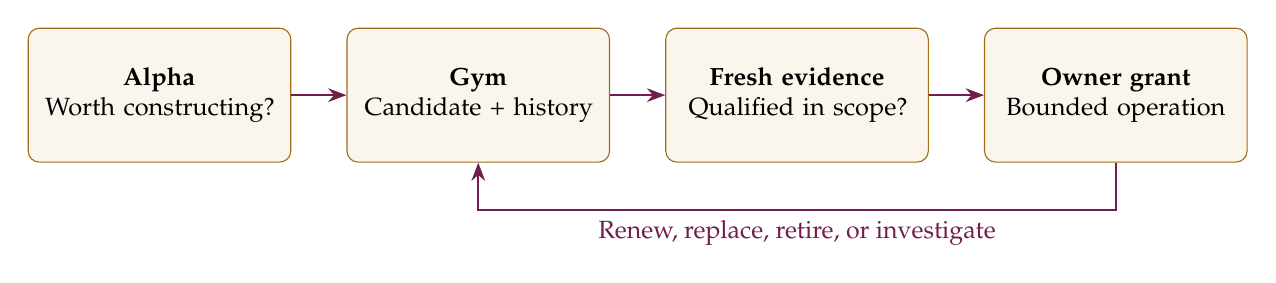
\begin{tikzpicture}[node distance=7mm,box/.style={draw=gold,fill=cream,rounded corners,align=center,text width=3.1cm,minimum height=17mm,font=\small},arr/.style={-{Stealth},thick,color=wine}]
\node[box] (a) {\textbf{Alpha}\\Worth constructing?};
\node[box,right=of a] (g) {\textbf{Gym}\\Candidate + history};
\node[box,right=of g] (s) {\textbf{Fresh evidence}\\Qualified in scope?};
\node[box,right=of s] (o) {\textbf{Owner grant}\\Bounded operation};
\draw[arr] (a)--(g);\draw[arr] (g)--(s);\draw[arr] (s)--(o);
\draw[arr] (o.south) -- ++(0,-.6) -| node[pos=.25,below,font=\small]{Renew, replace, retire, or investigate} (g.south);
\end{tikzpicture}
\caption{The four-stage vocabulary is implemented through distinct decisions. The development environment does not certify itself; evidence does not issue its own operating permission.}
\end{figure}

\section{Preserve the knowledge; renew the warrant}
\label{sec:evidence}
Let a qualification context be
\begin{equation}
 c=(m,s,v,e,q,p),
\end{equation}
where the entries identify the mission, source material, supplier configuration, environment, evaluator, and policy. A practical implementation must bind the complete executable dependency closure: prompts, adapters, libraries, tool versions, retrieval state, and relevant configuration, not only a short model name. The six strings in our local witness stand for that closure; they do not discover it.

A current evidence record binds a context digest, supported actions, validity interval, test protocol, and outcome. An authority record additionally binds an owner decision, an allowed action set, and its own validity interval. A historical record says what was established under its original conditions. It is not rewritten when current qualification expires.

\begin{definition}[Succession without privilege inheritance]
A restoration or successor initialization may import authorized knowledge, executable artifacts, and historical records. It initializes current evidence and active authority to empty. New operation requires an accepted context-bound qualification and a separate explicit grant.
\end{definition}

This conservative default does not prohibit efficient reuse. A validated generic check may remain applicable when its artifact, dependencies, checker, and environmental assumptions are unchanged. Current mission inputs, outputs, and material acceptance requirements still require current checks. A justified equivalence relation can reduce redundant work; a cache key alone cannot establish semantic equivalence.

\begin{proposition}[Context-bound action invariant]
\label{prop:authority}
Suppose every external action is mediated by a monitor that requires both a passing evidence record and an unexpired explicit grant, binds both to the current context, restricts the grant to the supported evidence scope, and clears the grant whenever qualification is replaced or revoked. If initialization and restoration create neither record, every permitted action is supported and authorized in its current recorded context and interval.
\end{proposition}

\begin{proof}
Initialization permits no action. Qualification alone creates no grant. A valid authorization transition creates only a subset of the supported actions, in the same context and within the evidence interval. The action check requires those predicates at the time of use. Replacement clears the grant; a context change fails the identity check; expiry or revocation fails the temporal or grant check. Induction over the permitted transitions establishes the invariant. This is a property of the specified monitor, not a proof that its evidence is truthful or that an implementation cannot be bypassed.
\end{proof}

\subsection{The assurance system is itself fallible}
A hash establishes byte identity under its cryptographic assumptions; it does not establish that the bytes describe the right physical object. Distinct role names do not establish independent organizations, independent model errors, or uncompromised storage. A source can be consistently wrong. A test population can omit the failure that matters. An honest verifier can have an incomplete specification.

The production design therefore needs threat modeling, complete mediation, authenticated owner decisions, isolation of protected evaluations, dependency integrity, recovery tests, and independent validation of evidence semantics. These requirements belong in implementation qualification. The NIST AI Risk Management Framework provides a relevant governance and lifecycle precedent, without turning our local prototype into certified compliance \citep{nistRMF}.

The same discipline applies to the Gym. Builder-generated tests can improve development. They cannot become the final judge merely because they favor the builder. Exposed confirmation cases become development material, not a fresh test set for the next renamed candidate. Repeated attempts consume a declared programme-wide error allocation when statistical claims are made.

\subsection{Three records, three different questions}
A useful implementation keeps a knowledge record, an evidence record, and an authority record conceptually separate. The first answers what the institution can legitimately reuse. The second answers what has been established for this context. The third answers what the owner has actually permitted. A fourth, financial record determines whether the action can be funded without consuming protected obligations.

None is a substitute for another. Scientific correctness cannot create a customer contract. A customer contract cannot establish physical performance. A large balance cannot grant access. A successful delivery cannot retroactively erase an invalid experiment. Institutional continuity consists partly of retaining these distinctions when components and personnel change.

\section{Renewal-adjusted Alpha}
\label{sec:alpha}
Let $\pi$ be a complete construction and operating policy over horizon $H$. Let $Y_t$ be accepted outcomes and $C_t$ the costs and losses actually incurred or explicitly modeled at time $t$. For a declared mission utility $U$ and discount factors $d_t$, define
\begin{equation}
 J_H(\pi)=\E\!\left[\sum_{t=0}^{H-1}d_t\{U(Y_t)-C_t\}-d_H O_H\right],
\end{equation}
where $O_H$ is the remaining terminal obligation under a stated valuation convention. Monetary costs and nonmonetary utility must be converted only through an explicit owner-approved decision model, or retained as separate constrained objectives.

For a frozen family $\mathcal B$ of credible complete alternatives,
\begin{equation}
 \alpha_H(\pi)=J_H(\pi)-\sup_{b\in\mathcal B}J_H(b).
 \label{eq:alpha}
\end{equation}
We call this \emph{renewal-adjusted Alpha} when the policies and their costs explicitly include replacement, migration, requalification, downtime, maintenance, and retirement, as well as initial development and operation. The expression is a decision criterion. An estimate of it is not established advantage, and a maximum over a finite supplied family is not a global economic optimum.

\subsection{Renewal can reverse a local ranking}
Suppose one specialist produces greater contribution on each active period but must be reconstructed whenever its supplier changes. A portable capability produces slightly less contribution but can be requalified at lower cost. A one-period comparison favors the specialist. A complete horizon may favor the portable capability. The decisive object is the supported productive trajectory, not the component's isolated score.

Conversely, portability can be wasteful. Its setup cost may never be recovered. The environment may not change. Retained assets may demand expensive maintenance. A new supplier may be incompatible with the supposed abstraction. An ordinary direct method may dominate. The institution should discover when to build continuity and when not to pay for it.

\subsection{Cash is a constraint, not a synonym for profit}
Let $B_t$ be cash before a period, $u_t$ its upfront payment, $r_t$ a receipt collected only after accepted delivery, and $\rho_t$ a protected reserve. In the finite study,
\begin{equation}
 B_t-u_t\geq\rho_t,\qquad B_{t+1}=B_t-u_t+r_t.
 \label{eq:cash}
\end{equation}
The first inequality is checked before collection. The second cannot make an unaffordable action valid retroactively. A positive horizon surplus does not establish that the policy can be started.

The study reports \emph{net cash surplus}, not accounting profit. There is no debt, equity issuance, receivable, tax model, salvage value, or noncash asset valuation. All cash flows are supplied by the fixture. Actual enterprise reporting must additionally reconcile accrual profit, liabilities, taxes, capital expenditures, and unrestricted cash without double-counting them. Agent development consumes actual resources; the absence of a human employee is not the absence of cost. Human labor is charged when it occurs, not inserted as a universal requirement.

\subsection{Value capture is a separate construction problem}
An owner needs both a useful capability and a voluntary route to receiving enough value to sustain it. Buyers can decline, use another provider, or perform the work themselves. Suppliers can change terms. Competitors can imitate. Owning a portable institution may reduce switching exposure, but its commercial benefit must survive real prices and actual behavior.

The appropriate contract might sell accepted outcomes, continuity of a bounded business function, a qualified instrument, or a separately priced renewal service. These are hypotheses, not measured demand. Customer data and methods do not become the provider's transferable property merely because they could improve another institution. A federation of institutions should exchange only permitted artifacts and evidence, with independent grants on each side.

The durable advantage we seek is the ability to keep constructing worthwhile capabilities, not a permanent monopoly margin. The previous FLYWHEEL $\Omega$ counterexample already shows why pricing claims must follow the choices participants can actually compose \citep{boucherFlywheel}. Institutional ownership adds another strategic choice: the ability to leave a supplier without abandoning the mission.

\section{An exact study of the institution that survives replacement}
\label{sec:study}
The study is a deliberately small, fully enumerable construction. Its purpose is to expose a lifecycle mechanism and its failure conditions. We supply the capabilities, contributions, replacement schedule, and action vocabulary. No model discovers these primitives; no customer purchases anything. The experiment tests exact planning, cash feasibility, and the consequences of retaining a useful artifact under those assumptions.

\subsection{The frozen environment}
There are 16 periods, divided into four supplier epochs of length four. Opening cash is 100 and the protected reserve is 20. The period is an abstract decision interval, not a month or a year. Each period permits one action. Payment precedes any collection. Development, renewal, and retirement consume a period during which no service is delivered.

The institution begins with a legacy service already qualified and available to every arm. That endowment is deliberate: the comparison does not charge the baseline an invented setup burden. A provider-specific specialist can be constructed for 40 units. A portable capability can be constructed for 60 units and incurs one unit of maintenance in every period in which it is retained, including its construction and renewal periods.

\begin{table}[htbp]
\centering\small
\caption{Supplied nominal action contracts. Maintenance is additional when the portable asset is retained. All values are abstract cash units, not measured prices.}
\begin{tabularx}{\textwidth}{@{}lrrX@{}}
\toprule
Action & Upfront & Receipt & Availability and effect\\
\midrule
Legacy delivery & 10 & 22 & Initially available; contribution 12.\\
Build specialist F & 40 & 0 & Qualifies F for the current supplier epoch.\\
Deliver with F & 12 & 42 & Requires current F qualification; contribution 30.\\
Build portable P & 60 & 0 & Retains P and qualifies it for the current epoch.\\
Deliver with P & 10 & 38 & Requires current P qualification; contribution 28 before maintenance.\\
Renew P & 10 & 0 & Retained P receives current-epoch qualification.\\
Idle & 0 & 0 & Maintenance still applies if P is retained.\\
Retire P & 0 & 0 & Removes P and future upkeep; no salvage receipt.\\
\bottomrule
\end{tabularx}
\end{table}

At a supplier change, current specialist and portable qualifications expire. The portable artifact remains available for renewal; the provider-specific specialist must be rebuilt. That difference is an authored property of the two contracts. It is not a measured universal property of portable versus provider-specific AI. Constructing a usable portability layer in a real system is precisely what the proposed industrial experiment must establish.

The complete state is $(t,B,o,e_P,e_F)$: period, cash, whether P is retained, and the epochs for which P and F are qualified. Qualification expires implicitly when an epoch identifier differs from the current epoch. The optimizer can choose the legacy service, build or use either specialist, retain or retire P, renew it, or idle. It is allowed to choose neither new capability.

All modeled service deliveries succeed and collect their specified receipt in the same period when demand is enabled. The default schedule is deterministic and known. There are no material capacity limits beyond one action per period, and no uncertain physical effects. These strong assumptions make the result exactly checkable; they also limit its commercial interpretation.

\subsection{Four comparisons, not a protected protagonist}
The \emph{full-option planner} has all actions. The \emph{no-portable planner} has the same cash rules and may rebuild F, use legacy, or idle; it tests the value of adding the supplied portable construction. The \emph{legacy-only control} uses the initial service or idles. Finally, an \emph{ordinary equal-content planner} has the same full action set and information. It reaches the same optimum. The ordinary control is not prohibited from retaining knowledge or constructing a portability layer.

We also evaluate a supplied \emph{always-retain policy}: immediately build P, renew it at each epoch change, and otherwise deliver with it. This policy is not allowed to borrow. It returns infeasible when it cannot prefund a required action. Its purpose is to test the tempting but incorrect rule that institutional continuity should always be purchased.

\subsection{Result: the stronger local component loses the horizon}
\begin{table}[htbp]
\centering
\caption{Nominal exact result. The 100-unit initial balance is not revenue. The 20-unit reserve remains inside terminal cash.}
\begin{tabular}{@{}lrrrr@{}}
\toprule
Policy & Collections & Outflows & Final cash & Cash surplus\\
\midrule
Legacy only & 352 & 160 & 292 & 192\\
Best without P & 504 & 304 & 300 & 200\\
Full option set & 456 & 226 & 330 & 230\\
Ordinary equal-content & 456 & 226 & 330 & 230\\
\bottomrule
\end{tabular}
\end{table}

The nominal full-option policy builds P in period zero, delivers three times, then renews and delivers three times in each subsequent epoch. The no-portable optimum builds F at the start of each epoch and delivers three times. P has lower active-period contribution, yet retains 30 more cash units over the complete horizon. Its 230-unit surplus is 15\% higher than the 200-unit no-portable surplus, \emph{within this fixture}. This is not a measured business margin or an AI productivity estimate.

The result has a useful second interpretation. The winning route collects \emph{less} revenue: 456 rather than 504. It wins because it spends less on reconstructing the means of delivery. Maximizing transaction value, isolated performance, or gross collections would not by itself identify the better funded trajectory.

\begin{figure}[htbp]
\centering
\begin{tikzpicture}
\begin{axis}[width=.96\textwidth,height=6.2cm,xlabel={Completed periods},ylabel={Cash units},xmin=0,xmax=16,ymin=0,ymax=350,xtick={0,4,8,12,16},ytick={0,100,200,300},grid=major,grid style={gray!15},legend style={at={(.02,.98)},anchor=north west,font=\small,draw=none,fill=white},tick label style={font=\small},label style={font=\small}]
\addplot[very thick,color=gold] table[x=t,y=portable,col sep=comma]{cash.csv};\addlegendentry{Full option set}
\addplot[thick,color=wine,dashed] table[x=t,y=no_portable,col sep=comma]{cash.csv};\addlegendentry{Best without P}
\addplot[thin,color=muted,dotted] table[x=t,y=legacy,col sep=comma]{cash.csv};\addlegendentry{Legacy only}
\addplot[gray,thin,domain=0:16] {20};
\end{axis}
\end{tikzpicture}
\caption{The exact cash paths, including construction and renewal interruptions. No future collection pays for its own upfront cost. The horizontal line marks the protected reserve.}
\end{figure}

\subsection{The crossover is explicit}
For a fixed sequence of $n$ complete epochs of length $L$, suppose rebuilding costs $D$, portable construction costs $B$, renewal costs $R$, and upkeep is $m$ per period. Let $g_F$ and $g_P$ be active-period contributions before portable upkeep. Each construction or renewal consumes one period. Conditional on financing both sequences,
\begin{align}
 S_F(n)&=n[(L-1)g_F-D],\\
 S_P(n)&=n(L-1)g_P-B-(n-1)R-nLm.
\end{align}
Hence
\begin{equation}
 S_P-S_F=n\underbrace{[(L-1)(g_P-g_F)+D-R-Lm]}_{\text{per-epoch continuity benefit}}-B+R.
 \label{eq:crossover}
\end{equation}
This is a comparison of two specified sequences, not proof that either is optimal in every environment. The exact planner establishes the nominal optimality separately.

With the nominal parameters, $S_P-S_F=20n-50$. P loses by 30 in one epoch, loses by 10 in two, wins by 10 in three, and wins by 30 in four. The advantage is created by repeated avoided reconstruction. It is not a mysterious multiplier of intelligence.

\begin{insight}[A distinction worth remembering]
The best component is not necessarily the best institution. The best institution is not necessarily the most persistent one. Preserve a capability only when its supported future uses justify construction, renewal, and upkeep.
\end{insight}

\subsection{The sensitivity study includes losses and non-entry}
Before executing the grid, the protocol fixed horizons $H\in\{8,12,16\}$, epoch lengths $L\in\{4,8\}$, opening cash $C\in\{40,70,100\}$, renewal costs $R\in\{5,10,25\}$, and upkeep $m\in\{0,1,3\}$. Their Cartesian product contains 162 environments. Both optimizers were checked against independently implemented forward reachability in every environment: 324 exact comparisons.

Adding the portable option strictly improves terminal cash in 19 environments and ties in 143. The largest gain is 61 units. There are no negative optimum differences because the full feasible set contains the no-portable set. \emph{That nonnegativity is a mathematical inclusion property, not evidence of robust positive treatment effects in a population of businesses.} The grid is supplied, not sampled from a real market.

Forced retention performs much worse: it is infeasible in 108 environments, loses to the no-portable optimum in 43, wins in 11, and ties in none. Infeasibility is an outcome, not a missing observation. These counts show why the institution must retain the option to delay, simplify, retire, or decline.

\begin{table}[htbp]
\centering\small
\caption{Predeclared diagnostic cases. Values are terminal cash; opening cash changes where stated. The full planner is free not to construct P.}
\begin{tabularx}{\textwidth}{@{}Xrr@{}}
\toprule
Changed condition & Full & Without P\\
\midrule
No supplier turnover during 16 periods & 510 & 510\\
No demand and no obligation to build & 100 & 100\\
Portable upkeep rises to 5 & 300 & 300\\
Portable renewal rises to 40 & 300 & 300\\
Opening cash is only the reserve, 20 & 20 & 20\\
Opening cash is 40 & 238 & 238\\
Horizon is one four-period epoch & 150 & 150\\
\bottomrule
\end{tabularx}
\end{table}

With no turnover, the higher-contribution F route wins. With opening cash equal to the reserve, even a profitable legacy delivery cannot be prefunded. With a four-period horizon, the always-portable sequence ends at 120 while the optimum ends at 150. The favorable nominal result does not license an unconditional preference for portability.

\subsection{Independent computation and its limits}
The primary solver uses memoized backward induction. The second implementation enumerates all reachable states forward and re-specifies action effects independently, without calling the primary transition function. The two implementations agree on every registered grid comparison. They share the authored specification and constants; agreement cannot validate those economic assumptions.

The companion also contains 35 unit tests covering planning and a local qualification/authority state machine. The latter preserves knowledge across export and restoration while rejecting inherited active proof or authority. Tests exercise changed context fields, expiry, revocation, unsupported actions, and missing owner approval. They establish behavior of this local software, not a hardened permission service or independent certification.

The implementation limit of 32 periods is a declared finite test boundary, not a business-scale ceiling. No live frontier-model calls, real customer data, actual collections, or physical operations occur. CPU time spent on publication and software construction is not hidden inside the abstract model's cash values. The supplied build, renewal, and maintenance prices are model inputs, not measured complete costs of this research programme.

\section{What must remain renewable}
\label{sec:renewal}
Useful capability is not merely installed capability. It must remain technically applicable, adequately evidenced, permitted, and affordable. This creates a renewal problem even when the underlying code remains unchanged.

\subsection{Renewal is a capacity constraint}
Suppose each deployed unit requires a current certificate, each certificate supports at most $\tau$ units of time, and the verification system can issue at most $v$ such unit-certificates per unit time. Let $B_0$ denote initially available remaining certified unit-time. For a horizon of length $T$, authorized productive unit-time is bounded by
\begin{equation}
 \int_0^T N_{\mathrm{active}}(t)\,dt\leq B_0+\tau vT.
 \label{eq:renewal}
\end{equation}
Thus long-run average authorized deployment cannot exceed $\tau v$ under these assumptions. Adding unqualified machines does not remove that bound.

This is a counting bound for a declared certification policy, not a physical law. A valid shared proof, a better production process, or a different independently justified validation architecture can change the unit of certification, $\tau$, or $v$. The productive invention may be the construction that makes those changes legitimate. It is not the deletion of the requirement while pretending reliability has been preserved.

\subsection{Invent the renewal mechanism}
A recurrent qualification burden can be approached in several ways. Improve the test. Construct an interface that makes irrelevant changes unable to affect the protected property. Preserve evidence during production so it need not be reconstructed afterward. Replace a fragile dependency. Or determine that full replay remains cheaper than maintaining a specialized reuse mechanism.

These routes transform the conditions under which intelligence becomes useful. The right target is not the minimum number of checks. It is the lowest complete burden of maintaining the required accepted outcome, including missed failures and the cost of invalidating stale conclusions.

A proof-producing interface may have large enabling value because many successors can use it. That does not make its value infinite. Integration, dependency tracking, compatibility testing, and obsolescence consume resources. The institution must compare its continued use with a clean rebuild and with simpler direct methods.

\subsection{A renewal reserve is not a growth forecast}
The operational reserve in the toy model is a supplied constant. A real institution needs a justified policy for existing obligations, rollback, incident response, and expected renewal work. Protecting those funds can prevent reinvestment even when accounting profit is positive. That is a cash decision, not a reason to erase the profit result.

Likewise, available cash does not establish an attractive next project. The proposed investment must identify what will be built, what independent acceptance would establish, when cash will be consumed, which liabilities remain, and why the complete route is preferable to alternatives. If these conditions fail, preserving optionality can be the better action.

\section{The institution must improve more than its inventory}
\label{sec:discovery}
The numerical study establishes the value of a supplied retention option in particular environments. It does not establish that a machine has become better at inventing that option. This boundary is central to the next research step.

Prior research supplies substantive but bounded precedents. DreamCoder jointly develops reusable program abstractions and search machinery in evaluated synthesis domains \citep{dreamcoder}. Enhanced POET studies the generation of challenges and solutions with transfer between environments \citep{poet}. Automated Design of Agentic Systems constructs executable agent designs rather than selecting only a fixed workflow catalogue \citep{adas}. AlphaEvolve uses generated code and automated evaluation for scientific and algorithmic discovery \citep{alphaevolve}. The Darwin Godel Machine explores an archive of self-modifying coding agents \citep{dgm}. These works motivate component mechanisms; none is evidence for the complete customer-owned, economically sustained, physically expanding institution proposed here.

\subsection{Three levels of inheritance}
A retained \emph{artifact} gives a successor a tool. A retained \emph{applicability model} helps determine where the tool is appropriate. A retained \emph{constructor} generates related tools under new conditions. The transition between each level is a separate empirical claim.

A failed transfer can be as informative as a success. It may show that the analogy was invalid, identify the missing interface, or reveal that the original objective does not actually need the assumed dependency. Negative evidence must retain its scope. Failure within one budget is not proof of universal impossibility; a success in one mission is not universal qualification.

The most ambitious inheritance is a better procedure for discovering constructors. It must be evaluated as a discovery policy, not inferred from the quality of one descendant. Replacing a costly committee with one good discriminating experiment can be an improvement. Architectural complexity is not the objective.

\subsection{The crossed experiment}
Let $\eta_0,\eta_1$ be earlier and revised discovery procedures, and $K_0,K_1$ earlier and updated starting capabilities. Evaluate all four combinations on genuinely fresh mission campaigns:
\begin{center}
\begin{tabular}{@{}lll@{}}
\toprule
 & Earlier capabilities $K_0$ & Updated capabilities $K_1$\\
\midrule
Earlier procedure $\eta_0$ & Reference & Inherited-equipment benefit\\
Revised procedure $\eta_1$ & Discovery-policy benefit & Combined effect\\
\bottomrule
\end{tabular}
\end{center}

Each arm receives comparable permissions and complete budgets. Strong unrestricted conventional construction and ordinary equal-content reuse remain available controls. Count the historical cost of acquiring the proposed improvement as well as its new campaign cost. The comparison unit for a claim about discovery is the complete campaign, not thousands of correlated substeps presented as independent replications.

An intervention is promoted only for the scope and claim that the evidence supports. A useful artifact can be adopted without proving improved discovery. A profitable business can expand without improving its intelligence. Conversely, a valuable scientific instrument may deserve a bounded research investment before it generates revenue. Keeping these cases separate allows ambition without a fictional universal success gate.

\subsection{The research executive can outgrow this paper}
The four-stage vocabulary is a public map, not a permanent grammar of intelligence. An effective institution may find a new representation, a different sequence of experiments, a simpler commercial arrangement, or a better way to allocate search. Its own route to improvement should remain revisable under the same protected purpose and evidence rules.

A genuine advance changes what becomes discoverable, constructible, verifiable, or economically deliverable. A new name for a fixed workflow does not. The complete mechanism must be executable and its contribution must survive a comparison in which the alternative is allowed to be competent.

\section{From productive surplus to a physical frontier}
\label{sec:physical}
An institution of intelligence becomes consequential at civilization scale only if its work changes what people can actually produce, understand, and sustain. Financial wealth is one means of coordination. It is not energy, a functioning factory, a validated material, or a beneficial outcome.

The proposed path has distinct links:
\begin{equation*}
\text{accepted value}\ \longrightarrow\ \text{available earned resources}\ \longrightarrow\ \text{qualified construction}\ \longrightarrow\ \text{commissioned capacity}.
\end{equation*}
Knowledge can strengthen every link, but cannot make the links identical. The earlier production-frontier paper explicitly distinguishes these quantities \citep{boucherFrontier}. SUCCESSOR $\Omega$ adds the requirement that the institution responsible for them remain capable of renewal across component generations.

\subsection{An auditable conversion contract}
For an investment $x$, define a proposed capacity-conversion contract
\begin{equation}
 \mathcal C_x=(Y_x,P_x,F_x,Q_x,T_x,R_x),
\end{equation}
where $Y_x$ is the intended physical output; $P_x$ the production and dependency plan; $F_x$ the timed funding and obligation schedule; $Q_x$ the independent qualification route; $T_x$ construction, integration, and deployment timing; and $R_x$ repair, renewal, retirement, and residual obligations. A project becomes commissioned capacity only when the relevant output and acceptance have actually occurred.

This contract is not a new financial instrument or a claim of available counterparties. It is a research and operating record. It prevents a forecast of future inventions from entering the ledger as installed machinery, and prevents a purchase commitment from entering it as available cash. Failed projects retain their costs even when the portfolio changes direction.

\subsection{The frontier is constrained by complementary flows}
If each commissioned unit requires material $a$, manufacturing work $b$, test capacity $c$, and deployable funding $d$, then a simplified steady-flow bound is
\begin{equation}
 \dot N\leq\min\left\{\frac{\dot M}{a},\frac{\dot W}{b},\frac{\dot Q}{c},\frac{\dot F}{d}\right\}.
 \label{eq:physicalcut}
\end{equation}
Units and time horizons must be compatible. The equation omits inventories, delays, reliability, resource substitution, and network topology; a detailed design must restore them. Its purpose is to expose the error of extrapolating one growing resource while ignoring the complementary requirements.

An intelligence can attempt to change a denominator, construct another route, increase a limiting throughput, or design a process that eliminates a requirement. It cannot assume that the change has occurred. Financial reinvestment with no material-processing capacity may accumulate claims rather than productive machinery. Manufacturing with inadequate acceptance capacity may accumulate uncommissioned inventory.

An expanding institution should therefore select inventions partly by which consequential bottleneck they remove. It should also ask whether the bottleneck moves elsewhere after the change. The best next invention can be a measurement, a production interface, or a coordination arrangement rather than the most visibly sophisticated component.

\subsection{A stellar-scale horizon, stated in physical units}
The distant research horizon is a productive civilization able to use a substantial fraction of stellar energy while preserving safety, legitimacy, and human benefit. This is an ambition to organize research, not a capability delivered by this paper or a date predicted by its model.

The IAU nominal solar luminosity is $L_\odot^{\mathrm N}=3.828\times10^{26}\,\mathrm W$; its nominal solar irradiance is $S_\odot^{\mathrm N}=1361\,\mathrm{W\,m^{-2}}$ \citep{iau}. These are nominal conversion constants, not claims about the Sun's exact instantaneous output. With intercepted fraction $f$, conversion efficiency $\eta$, and those reference values,
\begin{equation}
 P_{\mathrm{use}}=\eta fL_\odot^{\mathrm N},\qquad
 A_{\mathrm{collector}}\geq\frac{fL_\odot^{\mathrm N}}{S_\odot^{\mathrm N}}.
 \label{eq:stellar}
\end{equation}
The area is a simplified effective intercepting area at the reference irradiance. It assumes ideal orientation and no overlap or shading. It is not the surface area of a realizable structure.

For illustration only, take $f=10^{-12}$ and $\eta=0.30$. The intercepted power is $3.828\times10^{14}\,\mathrm W$, useful power is $1.1484\times10^{14}\,\mathrm W$, and effective collecting area is approximately $2.81\times10^{11}\,\mathrm{m^2}$, or 281,264 square kilometres. An assumed areal mass of $1\,\mathrm{kg\,m^{-2}}$ would already imply approximately $2.81\times10^{11}\,\mathrm{kg}$ of collector material alone. Neither efficiency nor areal mass is a demonstrated design in this programme.

Heat rejection creates another explicit requirement. Under a deliberately simplified cold-background radiator model,
\begin{equation}
 A_{\mathrm{radiating}}\geq\frac{P_{\mathrm{waste}}}{\epsilon\sigma T^4},
 \label{eq:heat}
\end{equation}
where $\sigma\simeq5.670374419\times10^{-8}\,\mathrm{W\,m^{-2}\,K^{-4}}$ \citep{nistSigma}. Taking $T=300\,\mathrm K$, emissivity $\epsilon=0.9$, and $P_{\mathrm{waste}}=0.7fL_\odot^{\mathrm N}$ gives approximately $6.48\times10^{11}\,\mathrm{m^2}$ of emitting area for the same illustrative fraction. This is total radiating area, not automatically the footprint of a one- or two-sided panel. Background radiation, solar heating, view factors, transport, degradation, and the eventual dissipation of useful energy are not modeled.

\begin{insight}[Why keep the physical arithmetic?]
Even a trillionth of a star's nominal luminosity implies a vast material, thermal, manufacturing, and coordination problem. A forecast of compounding money is not a construction plan for it. The opportunity is to invent the successive means that make each genuine step buildable.
\end{insight}

\subsection{Human benefit is not measured in watts alone}
Greater capacity can improve health, scientific access, resilience, and material well-being. It can also create concentrated power, ecological damage, or catastrophic exposure. The mission must therefore preserve explicit constraints on harm, distribution, consent, and accountability instead of assuming that greater throughput is inherently beneficial.

A customer-owned institutional design should make control and exit practical rather than concentrating authority in an irreplaceable supplier. At larger scales, coordination among independent institutions must remain permissioned, contestable, and subject to applicable public governance. The architecture is not a proposal for one autonomous owner to acquire unbounded authority. Greater capability increases the importance of justified limits and recoverable operation.

\section{The next consequential programme: an Industrial Requalification Foundry}
\label{sec:programme}
The proposed flagship is a foundry that constructs \emph{portable, independently testable industrial capabilities} across changing instruments, model providers, and operating conditions. The intended outcome is not another evaluation dashboard. It is reduced lifecycle burden for useful scientific and industrial work that currently loses too much value at each transition.

An initial candidate mission is evidence-preserving experimental planning for battery-process qualification. The institution would connect source-grounded materials knowledge, simulation, experimental design, measured manufacturing variation, acceptance tests, and renewal after an instrument or supplier change. This is a candidate, not a market selection already established by data. Other missions may offer greater consequence or a sharper initial test.

\subsection{Construct a missing means, not a narrative}
One prospective instrument is a \emph{renewal-aware experiment compiler}. It would map a proposed configuration change to the claims potentially affected, preserve justified unchanged evidence, construct the smallest discriminating experiments needed for new claims, and produce an executable qualification plan with complete costs. The plan can conclude that the dependency closure is unknown or that a clean rebuild is preferable.

The critical inventive step is constructing the mapping from changes to consequential claims, not merely sorting a supplied dependency graph. A prototype that receives every causal edge from its designer should be reported as a supplied-graph implementation. An autonomous discovery claim requires the system to infer or construct missing structure and test it against protected cases.

A second prospective instrument would make work easier to qualify by construction: typed experimental interfaces, provenance-preserving observations, declared calibration contracts, and explicit failure behavior. That could change the amount of recurrent reasoning required. It also creates costs and new failure modes, which belong in the comparison.

\subsection{The first decisive campaign}
Start with one bounded mission and three materially different routes: a strong direct specialist; ordinary modular engineering with full documentation and reuse; and a candidate permitted to invent a new representation, experiment, or interface. All receive the same substantive source access, construction permissions, and complete campaign budget. The candidate must not receive an exclusive prebuilt connector.

Separate development cases from fresh confirmation. Include cases where the change is irrelevant, where a narrow test is sufficient, where complete replay is necessary, where a reference is coherently wrong, and where no affordable test justifies operation. Supplier replacement, source mutation, changed measurement semantics, and expired permission are different interventions and must not be collapsed into one generic drift score.

The primary endpoint is the cost and time to an independently accepted mission outcome, subject to fixed material quality and safety requirements. Report wrong approvals, false rejections, uncertainty, interruption recovery, and actual consumed resources. For a physical claim, a simulation result advances only to a justified physical test; it does not count as that test. The reserve for independent confirmation is protected before search begins.

Then test a fresh successor, such as another production line or measurement configuration. Compare inherited machinery with no inheritance and ordinary equal-content reuse. Finally, perform the crossed discovery-policy comparison from Section~\ref{sec:discovery}. These are three separate experiments, not three names for the same favorable run.

\subsection{The voluntary commercial bridge}
The buyer hypothesis is that a qualified institution can deliver a valuable bounded outcome and preserve the means of delivering it through future changes. Buyer acceptance must establish actual willingness to pay for that outcome relative to alternatives, not agreement with the vision. Proposed prices are experiments, not evidence of demand.

A pilot should record authorized onboarding, independently accepted work, actual collection, acquisition burden including declined offers, failures, renewal obligations, and unrestricted funds. Repeat purchase and portability after supplier replacement are separate observable outcomes. Commercial performance can be recognized without claiming improved invention; a technically impressive renewal method can be rejected when a simpler service produces greater complete value.

Physical expansion follows only through separately funded and qualified projects. A positive digital-service surplus may finance laboratory work. It does not establish that the laboratory work will succeed. An industrial result may enable another capability. That enabling relationship requires its own comparison, and the full lineage retains unsuccessful costs.

\section{Scope, failure modes, and what would falsify the thesis}
\label{sec:limits}
Our strongest established numerical claim is conditional: for the registered finite environments, the exact solver and the independent reachability implementation agree, and the nominal portable route has greater cash surplus than the best supplied no-portable route. The ordinary equal-content planner ties it. The state-machine tests establish local transition behavior. The physical arithmetic is a dimensional scale check. None is evidence of autonomous commercial success or a newly achieved level of intelligence.

The economic fixture gives P cheaper renewal by assumption. It does not estimate how often suppliers change, how well capabilities transfer, what buyers will pay, or the probability of qualification failure. Known future turnover is especially favorable to planning. A real implementation must confront uncertain change, collection delay, competing prices, obsolescence, multi-period experiments, and operational mistakes. The study's positive cases do not establish their prevalence.

The institutional hypothesis loses its practical value in a mission where the strongest ordinary arrangement already preserves equivalent capability at equal or lower complete cost. It also fails when export omits a decisive dependency, renewal produces stale assurance, maintenance absorbs the operating surplus, the owner cannot actually control the assets, or preserved machinery does not help fresh work. Those are substantive negative results, not reasons to weaken the comparator.

The broader recursive hypothesis requires more. A history of successful tools may still leave discovery unchanged. A revised search procedure can look better because it consumes more resources or sees confirmation material. A larger archive can make retrieval worse. The design must allow a simple conventional alternative to win and the incumbent to remain in service.

Finally, no general inference runs from intelligence to unlimited growth. Production needs physical resources, economic participation, infrastructure, time, and legitimate authority. A useful method can accelerate a link without establishing the entire chain. The programme should pursue the links that could have the greatest consequence, while reporting exactly which have been built and which remain hypotheses.

\section{Conclusion: build what can build beyond itself}
\label{sec:conclusion}
A successful answer is an output. A useful invention is a capability. An enduring institution preserves the legitimate means of producing further capabilities while remaining able to replace the components that once made it successful.

SUCCESSOR $\Omega$ puts that distinction into an economic and experimental form. Find an advantage worth constructing. Develop it in a mission environment. Make the claim survive fresh comparison. Grant bounded authority separately. Preserve what genuinely transfers, renew what must be current, and retire what no longer earns its cost.

The exact study demonstrates why the lifecycle matters: a lower-contribution portable capability can beat repeated reconstruction, yet continuity can also be unaffordable or inferior. Its ordinary equal-content tie identifies the actual mechanism without inventing superiority for a label. The research challenge is now to discover, build, and qualify such enabling arrangements in consequential missions.

The larger opportunity is to compound more than money or artifacts. It is to develop institutions whose work expands what can be investigated, constructed, delivered, and sustained---and whose earned resources help make the next genuine advance possible. Scientific instruments, industrial systems, and energy-producing capacity are destinations for that process, not numbers to be asserted in advance.

\begin{insight}[The governing ambition]
Own the institution. Replace the models. Preserve the mission.\\[3pt]
Make the next breakthrough easier to construct---without making its proof easier to evade.
\end{insight}

\clearpage
\appendix
\section{Formal details and boundary conditions}
\label{app:formal}
\subsection{Finite optimization}
For state $s_t=(t,B_t,o_t,e_{P,t},e_{F,t})$, let $\mathcal A(s_t)$ be the legal supplied actions satisfying the pre-collection reserve. Each action has deterministic cost $u(s_t,a)$, collection $r(s_t,a)$, and successor state $T(s_t,a)$. The primary recursion is
\begin{equation}
 V_H(s_H)=B_H,\qquad V_t(s_t)=\max_{a\in\mathcal A(s_t)}V_{t+1}(T(s_t,a)).
\end{equation}
The implementation breaks equal terminal-cash outcomes by lexicographic action-sequence order. That affects the selected trace, not the optimal cash value. Idle is feasible when no portable asset is retained. When upkeep is unaffordable, retirement remains feasible and consumes the period. Thus an admitted state always has a continuation.

\begin{proposition}[Exactness within the declared action set]
For the finite deterministic model, backward induction returns the maximum terminal cash over all reserve-respecting action sequences. Independent forward enumeration returns the same maximum when it uses the same transition specification.
\end{proposition}
\begin{proof}
At the terminal layer the value equals cash by definition. If continuation values at $t+1$ are exact, maximizing over every legal first action at $t$ examines every feasible sequence partitioned by that action. Induction proves the first statement. Forward enumeration starts from the admitted state and adds every legal successor at each period; induction identifies its layer with exactly the reachable state set. Taking maximum cash at the final layer proves the second. Agreement between implementations is a useful defect check, not evidence that the supplied model describes a market.
\end{proof}

\begin{corollary}[Option inclusion]
If $\mathcal A_0$ is a subset of $\mathcal A_1$ at every state and all common action effects, endowments, and constraints agree, the optimum under $\mathcal A_1$ cannot be lower.
\end{corollary}
\begin{proof}
Every feasible $\mathcal A_0$ action sequence is also feasible under $\mathcal A_1$. Maximization over the larger set contains the original maximum.
\end{proof}
This explains the absence of negative full-option differences. It does not protect the always-retain policy, which removes choices and pays costs even when they are not justified. Nor does it justify treating a preconstructed portability layer as free in a comparison of discovery systems.

\subsection{The renewal crossover}
If every epoch contains one construction or renewal period and $L-1$ active periods, F earns $(L-1)g_F-D$ per epoch. P earns $n(L-1)g_P$, pays its initial construction $B$, pays $n-1$ renewals, and pays $nL$ periods of upkeep. Subtraction gives Equation~\ref{eq:crossover}.

When $\Delta=(L-1)(g_P-g_F)+D-R-Lm>0$ and $B>R$, P strictly wins those fixed sequences when
\begin{equation}
 n>\frac{B-R}{\Delta}.
\end{equation}
The first strictly winning integer is $\lfloor(B-R)/\Delta\rfloor+1$. If $\Delta\leq0$, additional epochs do not create the same amortization advantage. Other signs of $B-R$ must be evaluated directly from the inequality, rather than forcing this positive-threshold interpretation.

Let $D_P^{\mathrm{extra}}$ and $D_F^{\mathrm{extra}}$ be additional total lifecycle burdens omitted from the toy contracts. Under a compatible monetary accounting convention, the nominal 30-unit difference survives only if $D_P^{\mathrm{extra}}-D_F^{\mathrm{extra}}<30$. Liquidity can fail even before that surplus threshold: the timing of an additional burden matters as well as its total. This sensitivity statement does not estimate those burdens.

\subsection{Prefix financing}
For an ordered cash sequence with constant reserve $\rho$, define the cumulative pre-collection deficit through action $j$ as
\begin{equation}
 D_j=\sum_{i=0}^{j}u_i-\sum_{i=0}^{j-1}r_i.
\end{equation}
The sequence is feasible exactly when its initial cash satisfies
\begin{equation}
 B_0\geq\rho+\max(0,\max_j D_j).
 \label{eq:prefund}
\end{equation}
\begin{proof}
Immediately before receipt $r_j$, cash equals $B_0-D_j$. Requiring this quantity to be at least $\rho$ for every $j$ is equivalent to the bound. The extra zero ensures the initial reserve itself is funded.
\end{proof}
For the nominal immediate P construction, the first payment is 61 including upkeep. Opening cash must therefore be at least 81 before this fixed route can begin. A different policy may first earn legacy receipts, delay construction, or choose F. Equation~\ref{eq:prefund} is a route-specific condition, not a universal minimum capital for the mission.

\subsection{Renewal-throughput bound}
Let certificates issued within $[0,T]$ each contribute at most $\tau$ authorized unit-time, and let at most $vT$ certificates be issued. Initial residual coverage is at most $B_0$. The union of covered productive unit-time cannot exceed the sum of these coverage budgets, yielding Equation~\ref{eq:renewal}. Overlap only makes the bound looser. Dividing by $T$ and taking a long horizon gives average active units at most $\tau v$ if $B_0/T\to0$.

A certificate covering a fleet is not a unit-certificate under this assumption. A validated fleet-level qualification changes the model and may improve the bound; an unsupported fleet-level assertion does not. Hardware construction throughput, material availability, and repair constraints can impose additional tighter bounds.

\section{The numerical record}
\label{app:record}
\subsection{Complete nominal route}
\begin{center}
\small
\begin{tabular}{@{}rrrrrr@{}}
\toprule
Period & Action & Opening & Paid & Collected & Closing\\
\midrule
\input{trace_rows.tex}
\bottomrule
\end{tabular}
\end{center}
The trace above is generated from the companion rather than copied from a plotted image. The publication build checks the terminal balance, collections, outflows, reserve, grid counts, and physical arithmetic before typesetting.

\subsection{Protocol history and stopping rule}
The finite economic protocol fixed the primary fixture, comparator permissions, 162-case grid, and qualitative adverse cases before numerical evaluation in this authoring session. It was an internal prospective record, not a timestamped independent preregistration. The one-epoch and 40-unit opening-cash diagnostic traces were added as explanatory checks; the latter setting is already in the frozen grid. No selection claim is made from those additions. A planned additional-burden check is reported algebraically in Appendix~\ref{app:formal}, rather than represented as a separately executed market experiment.

The stopping rule is completion of the registered grid, diagnostics, and regression suite. There is no search for a favorable random seed, no independent sample of businesses, and no confidence interval over an invented population. The final source is bound to its generated results and rerun during publication qualification. Source changes are visible in normal version control; the favourable nominal case is not relabeled as universal performance.

\subsection{Cost scope and interpretation}
The finite model includes exactly the listed payments, deterministic accepted collections, upkeep, and one-period construction and renewal delays. It excludes real customer acquisition, actual model-provider invoices, uncertainty in demand and qualification, tax and liability accounting, physical deployment, and the cost of creating this paper. Those exclusions are not estimates of zero. They prevent the experiment's cash surplus from being described as demonstrated complete-cost commercial profit.

The nominal initial 100 units are a fixture, not a mandatory dollar capitalization for AGI ALPHA. The programme can compare different initial financing, staged construction, cooperation, and non-entry, subject to actual authority and voluntary participation. The separate US\$3 billion trailing-365-day complete-cost profit objective is not achieved by this paper. Multiplying abstract units by a currency scale would not achieve it either.

\section{A claim ledger for the complete programme}
\label{app:claims}
\begin{longtable}{@{}p{.20\textwidth}p{.34\textwidth}p{.38\textwidth}@{}}
\toprule
Claim & Evidence in this edition & What it does not establish\\
\midrule
\endhead
Lifecycle reversal & Exact nominal policies, cash traces, and crossover identity. & Measured demand, actual prices, or autonomous invention.\\[5pt]
Finite optimality & Backward solver and independent forward enumeration agree on 324 grid comparisons. & Global optimality over unspecified strategies or markets.\\[5pt]
Optional retention & 19 positive differences and 143 ties; forced retention often loses or cannot start. & A frequency estimate for real-world portability benefits.\\[5pt]
Scoped action logic & Local tests of context, grant scope, expiry, revocation, and clean restoration. & Secure complete mediation, authentic identities, truthful evidence, or production certification.\\[5pt]
Institutional ownership & Export/restore semantics and proposed acceptance contract. & Legal rights to third-party assets or a deployed customer product.\\[5pt]
Inventive succession & Fresh-successor and crossed-policy experimental designs. & Demonstrated improvement of a discovery procedure.\\[5pt]
Commercial compounding & Explicit collection, obligations, and reinvestment requirements. & Actual customer profit or the programme's monetary milestone.\\[5pt]
Physical expansion & Conversion-contract framework, complementary-flow bounds, dimensional calculations. & A tested collector, radiator, factory, or industrial growth forecast.\\[5pt]
Stellar-scale capability & A long-horizon research objective with physical quantities exposed. & An achieved civilization level, an investment return, or a timetable.\\
\bottomrule
\end{longtable}

\section{Reproduce, inspect, extend}
\label{app:reproduce}
The companion requires Python 3.10 or later and the standard library. From the source directory:
\begin{verbatim}
python3 -m unittest -v test_companion
python3 companion.py --output results.json
python3 build.py --output /tmp/successor-publication
\end{verbatim}
The last command also needs a PDFLaTeX/BibTeX installation with the packages named in \texttt{paper.tex}, Poppler, and CairoSVG for the share image. It generates the cash data and trace table, compiles the paper, records tool versions and file hashes, and packages a deterministic source archive. The build uses a fixed source-date epoch and suppresses variable PDF metadata. Byte identity is checked in the recorded build environment; equivalent output across arbitrary TeX versions is not assumed.

The archive contains the manuscript, bibliography, public reader template, original vector share artwork, exact model, tests, protocol, and build tooling. It contains no private conversation documents, customer data, credentials, or copied model weights. The versioned GitHub edition provides the released PDF, source ZIP, and checksums. A source/PDF manifest binds the artifact to the source files that generated it.

To extend the study, create a new declared protocol rather than silently changing this edition's assumptions. Useful next variations include uncertain replacement time, qualification failure, delayed collection, multiple complementary capabilities, finite maintenance capacity, and actual measured migration costs. Any comparison claiming improved discovery must give conventional alternatives the same information and construction permissions.

\subsection*{Authorship and research assistance}
Vincent Boucher specifies the research direction and is the named author of this edition. AI-assisted synthesis, mathematical drafting, implementation, and publication tooling were used in its preparation. The finite model and its constants are authored inputs. Independent implementation of the reachability check is an algorithmic cross-check within this publication workflow, not independent external peer review or physical validation.

\bibliographystyle{plainnat}
\bibliography{references}
\end{document}
